\documentclass[11pt]{mimosis}
% \PassOptionsToClass{14pt}{scrbook}
\usepackage{metalogo}

\usepackage{textcomp}
\usepackage{gensymb}

%%%%%%%%%%%%%%%%%%%%%%%%%%%%%%%%%%%%%%%%%%%%%%%%%%%%%%%%%%%%%%%%%%%%%%%%
% Some of my favorite personal adjustments
%%%%%%%%%%%%%%%%%%%%%%%%%%%%%%%%%%%%%%%%%%%%%%%%%%%%%%%%%%%%%%%%%%%%%%%%
%
% These are the adjustments that I consider necessary for typesetting
% a nice thesis. However, they are *not* included in the template, as
% I do not want to force you to use them.

% This ensures that I am able to typeset bold font in table while still aligning the numbers
% correctly.
\usepackage{etoolbox}

\usepackage[binary-units=true]{siunitx}
\DeclareSIUnit\px{px}

\sisetup{%
  detect-all           = true,
  detect-family        = true,
  detect-mode          = true,
  detect-shape         = true,
  detect-weight        = true,
  detect-inline-weight = math,
}

%%%%%%%%%%%%%%%%%%%%%%%%%%%%%%%%%%%%%%%%%%%%%%%%%%%%%%%%%%%%%%%%%%%%%%%%
% Hyperlinks & bookmarks
%%%%%%%%%%%%%%%%%%%%%%%%%%%%%%%%%%%%%%%%%%%%%%%%%%%%%%%%%%%%%%%%%%%%%%%%

\usepackage[%
  colorlinks = true,
  citecolor  = Black,
  linkcolor  = Black,
  urlcolor   = Black,
  ]{hyperref}

\usepackage{bookmark}


%%%%%%%%%%%%%%%%%%%%%%%%%%%%%%%%%%%%%%%%%%%%%%%%%%%%%%%%%%%%%%%%%%%%%%%%
% Bibliography
%%%%%%%%%%%%%%%%%%%%%%%%%%%%%%%%%%%%%%%%%%%%%%%%%%%%%%%%%%%%%%%%%%%%%%%%
%
% I like the bibliography to be extremely plain, showing only a numeric
% identifier and citing everything in simple brackets. The first names,
% if present, will be initialized. DOIs and URLs will be preserved.

\usepackage[%
  autocite     = plain,
  backend      = bibtex,
  doi          = true,
  url          = true,
  giveninits   = true,
  hyperref     = true,
  maxbibnames  = 99,
  maxcitenames = 99,
  sortcites    = true,
  style        = alphabetic,
  citestyle    = alphabetic,
  backref      = true,
  ]{biblatex}


%%%%%%%%%%%%%%%%%%%%%%%%%%%%%%%%%%%%%%%%%%%%%%%%%%%%%%%%%%%%%%%%%%%%%%%%
% Some adjustments to make the bibliography more clean
%%%%%%%%%%%%%%%%%%%%%%%%%%%%%%%%%%%%%%%%%%%%%%%%%%%%%%%%%%%%%%%%%%%%%%%%
%
% The subsequent commands do the following:
%  - Removing the month field from the bibliography
%  - Fixing the Oxford commma
%  - Suppress the "in" for journal articles
%  - Remove the parentheses of the year in an article
%  - Delimit volume and issue of an article by a colon ":" instead of
%    a dot ""
%  - Use commas to separate the location of publishers from their name
%  - Remove the abbreviation for technical reports
%  - Display the label of bibliographic entries without brackets in the
%    bibliography
%  - Ensure that DOIs are followed by a non-breakable space
%  - Use hair spaces between initials of authors
%  - Make the font size of citations smaller
%  - Fixing ordinal numbers (1st, 2nd, 3rd, and so) on by using
%    superscripts

% Remove the month field from the bibliography. It does not serve a good
% purpose, I guess. And often, it cannot be used because the journals
% have some crazy issue policies.
\AtEveryBibitem{\clearfield{month}}
\AtEveryCitekey{\clearfield{month}}

% Fixing the Oxford comma. Not sure whether this is the proper solution.
% More information is available under [1] and [2].
%
% [1] http://tex.stackexchange.com/questions/97712/biblatex-apa-style-is-missing-a-comma-in-the-references-why
% [2] http://tex.stackexchange.com/questions/44048/use-et-al-in-biblatex-custom-style
%
\AtBeginBibliography{%
  \renewcommand*{\finalnamedelim}{%
    \ifthenelse{\value{listcount} > 2}{%
      \addcomma
      \addspace
      \bibstring{and}%
    }{%
      \addspace
      \bibstring{and}%
    }
  }
}

% Suppress "in" for journal articles. This is unnecessary in my opinion
% because the journal title is typeset in italics anyway.
\renewbibmacro{in:}{%
  \ifentrytype{article}
  {%
  }%
  % else
  {%
    \printtext{\bibstring{in}\intitlepunct}%
  }%
}

% Remove the parentheses for the year in an article. This removes a lot
% of undesired parentheses in the bibliography, thereby improving the
% readability. Moreover, it makes the look of the bibliography more
% consistent.
\renewbibmacro*{issue+date}{%
  \setunit{\addcomma\space}
    \iffieldundef{issue}
      {\usebibmacro{date}}
      {\printfield{issue}%
       \setunit*{\addspace}%
       \usebibmacro{date}}%
  \newunit}

% Delimit the volume and the number of an article by a colon instead of
% by a dot, which I consider to be more readable.
\renewbibmacro*{volume+number+eid}{%
  \printfield{volume}%
  \setunit*{\addcolon}%
  \printfield{number}%
  \setunit{\addcomma\space}%
  \printfield{eid}%
}

% Do not use a colon for the publisher location. Instead, connect
% publisher, location, and date via commas.
\renewbibmacro*{publisher+location+date}{%
  \printlist{publisher}%
  \setunit*{\addcomma\space}%
  \printlist{location}%
  \setunit*{\addcomma\space}%
  \usebibmacro{date}%
  \newunit%
}

% Ditto for other entry types.
\renewbibmacro*{organization+location+date}{%
  \printlist{location}%
  \setunit*{\addcomma\space}%
  \printlist{organization}%
  \setunit*{\addcomma\space}%
  \usebibmacro{date}%
  \newunit%
}

% Do not abbreviate "technical report".
\DefineBibliographyStrings{english}{%
  techreport = {technical report},
}

% Display the label of a bibliographic entry in bare style, without any
% brackets. I like this more than the default.
%
% Note that this is *really* the proper and official way of doing this.
\DeclareFieldFormat{labelnumberwidth}{#1\adddot}

% Ensure that DOIs are followed by a non-breakable space.
\DeclareFieldFormat{doi}{%
  \mkbibacro{DOI}\addcolon\addnbspace
    \ifhyperref
      {\href{http://dx.doi.org/#1}{\nolinkurl{#1}}}
      %
      {\nolinkurl{#1}}
}

% Use proper hair spaces between initials as suggested by Bringhurst and
% others.
\renewcommand*\bibinitdelim {\addnbthinspace}
\renewcommand*\bibnamedelima{\addnbthinspace}
\renewcommand*\bibnamedelimb{\addnbthinspace}
\renewcommand*\bibnamedelimi{\addnbthinspace}

% Make the font size of citations smaller. Depending on your selected
% font, you might not need this.
\renewcommand*{\citesetup}{%
  \biburlsetup
  \small
}

% \DeclareLanguageMapping{british}{bibliography-correct-ordinals}
% \DeclareLanguageMapping{english}{bibliography-correct-ordinals}
\bibliography{Thesis}

%%%%%%%%%%%%%%%%%%%%%%%%%%%%%%%%%%%%%%%%%%%%%%%%%%%%%%%%%%%%%%%%%%%%%%%%
% Fonts
%%%%%%%%%%%%%%%%%%%%%%%%%%%%%%%%%%%%%%%%%%%%%%%%%%%%%%%%%%%%%%%%%%%%%%%%

\ifxetexorluatex
  %\setmainfont{Minion Pro}
  \usepackage{microtype}
\else
  %\usepackage[osf,lining]{ebgaramond}  
  \usepackage[scale=0.7]{sourcecodepro}  
\fi






\usepackage{mathpazo}
\usepackage{lettrine}

\usepackage{makeidx}
\makeindex



\newacronym[description={Principal component analysis}]{PCA}{PCA}{principal component analysis}
\newacronym                                            {SNF}{SNF}{Smith normal form}
\newacronym[description={Topological data analysis}]   {TDA}{TDA}{topological data analysis}

%\makeindex
\makeglossaries

%%%%%%%%%%%%%%%%%%%%%%%%%%%%%%%%%%%%%%%%%%%%%%%%%%%%%%%%%%%%%%%%%%%%%%%%
% Incipit
%%%%%%%%%%%%%%%%%%%%%%%%%%%%%%%%%%%%%%%%%%%%%%%%%%%%%%%%%%%%%%%%%%%%%%%%

\newcommand*{\titleGP}{\begingroup % Create the command for including the title page in the document
\centering % Center all text
\vspace*{\baselineskip} % White space at the top of the page

%\rule{\textwidth}{1.6pt}\vspace*{-\baselineskip}\vspace*{2pt} % Thick horizontal line
%\rule{\textwidth}{0.4pt}\\[1.0\baselineskip] % Thin horizontal line

{\huge A Novel Tool for Multidimensional Online Discourse Visualization}\\[0.2\baselineskip] % Title

%\rule{\textwidth}{0.4pt}\vspace*{-\baselineskip}\vspace{3.2pt} % Thin horizontal line
%\rule{\textwidth}{1.6pt}\\ % Thick horizontal line

\vspace*{\baselineskip}

{\Large Advanced Practical\\[\baselineskip]} % Tagline(s) or further description
\vspace*{\baselineskip}

{\LARGE Rauls Florian\\[\baselineskip]} % Editor list  

\vspace*{\baselineskip} % Whitespace between location/year and editors

Supervisor\\
{\large  Prof. Dr. Filip Sadlo\\[\baselineskip]} % Editor list

\vfil

Heidelberg,  \today \par % Location and year

\vspace*{\baselineskip}

{\itshape Faculty of Mathematics and Computer Science\par} % Editor affiliation
{\itshape Heidelberg University\par} % Editor affiliation

\endgroup}

 
\usepackage{mathtools}
\usepackage{amssymb}
\usepackage{siunitx}

\usepackage{blindtext}

\usepackage{algorithm2e}

% Corrects \autoref{}: chapter -> Chapter, section -> Section, subsection -> Section
\addto\extrasenglish{%
  \renewcommand{\chapterautorefname}{Chapter}%
  \renewcommand{\sectionautorefname}{Section}%
  \renewcommand{\subsectionautorefname}{Section}%
}

\begin{document}

\frontmatter
\thispagestyle{empty}
  \titleGP  
  \cleardoublepage
  \pagestyle{empty}
  %\section*{Declaration of Authorship}

I hereby declare that the thesis submitted is my own unaided work. All direct or indirect sources used are acknowledged as references. The principles and recommendations \enquote{Verantwortung in der Wissenschaft} of Heidelberg University have been followed.
\vspace{5cm}\\
\noindent\rule[0.5ex]{8em}{0.5pt} \hfill \rule[0.5ex]{10em}{0.5pt}\\
\noindent first and last name \hfill city, date and signature
  \begin{center}
\abstract{
  We propose a novel tool for visualizing the flow of discussions over temporal, spatial, sentimental and other custom dimensions simultaneously, by utilizing meta-data which is contained in most messages written on wide-spread microblogging services. For this we built a pipeline, which can automatically collect and process messages posted on the popular social media network \emph{Twitter}, developed a scheme for presenting the diverse range of data points in such a way, that an user can understand and filter them intuitively and evaluated our approach by analyzing discussions which are contained in our dataset. We furthermore demonstrate on how to best use our software, by describing an example research scenario and give instructions on how to solve it. Our tool can be used for detailed analysis of conversations on social media platforms. Our tool can be used to answer questions, which might be raised about discussions online and development of conversations.
We also discuss issues which arise from different visualization schemes and how to tackle them in the future. 
 }
\end{center}
%
\noindent 


  \tableofcontents

\mainmatter
  \pagestyle{scrheadings}

  %%%%%%%%%%%%%%%%%%%%%%%%%%%%%%%%%%%%%%%%%%%%%%%%%%%%%%%%%%%%%%%%%%%%%%%%
\chapter{Introduction}

Microblogging services on social media platforms are rising in their popularity since their first appearance in the 2000s. Their importance is not only highlighted by the number of users which are using services like \emph{Twitter} daily, but also by being the center point of political discussions online. With this rise in importance, different research fields have been founded to analyze and understand behavioral patterns and information propagation inside them. Even though recent findings show that social networks are not representative of the overall population, ~\cite{mellon2017twitter} it is still important to understand the dynamics at play when working in fields like political science or communications. 

When short messages are posted online, many platforms provide some way of responding to any message for other users. A good example would be the \emph{retweet} feature on \emph{Twitter}. Any user can \emph{retweet} a message, therefore displaying the source to their followers, and in turn add their own message as a comment. This of course leads to chains of message, where often times discussions are held in the form of \emph{retweets} of \emph{retweets}. Even though one could easily follow a single chain of back and forth, any \emph{tweet} can have $n$ \emph{retweets}, which produces an ever-increasing complexity of threads to follow. 

We propose a visualization scheme for these discussion threads, where each message gets rendered at their temporal and spatial position, whilst message-answer-relations are indicated via pointers. Additional information like message \emph{sentiment} (tonal connotation) can be visualized through coloration, and distributions of any further dimensions can be shown in affixed plots right next to the rendered scene. Our dashboard also includes a graphical user interface, through which filters can be applied. Examples for filters could be maximum sentimental tone, usage of a so-called \emph{hashtag} or limitations in temporal occurrence. In combination, these tools enable users to narrow down messages to certain topics and any other desired specification. Complex research questions can be handled through these means, as one could e.g. ask \emph{"Does the tone of any given discussion get friendlier over time, when looking at the topic of school reforms?"}.
  %%%%%%%%%%%%%%%%%%%%%%%%%%%%%%%%%%%%%%%%%%%%%%%%%%%%%%%%%%%%%%%%%%%%%%%%
\chapter{Related Work}
\label{sec:relatedWork}
%%%%%%%%%%%%%%%%%%%%%%%%%%%%%%%%%%%%%%%%%%%%%%%%%%%%%%%%%%%%%%%%%%%%%%%%

Since social media and online discourse are very wide topics, with lots of points of interest, a lot of research went into different forms of discourse analysis. For once topic modeling on specific points of discourse, like done by~\cite{TORNBERG2016132}, who used topic modeling and critical discourse analysis to investigate the portrayal of Muslim communities online,  is very popular. 

For methods of visualization~\cite{mckelvey2012visualizing} are closely related to our approach, as they used diffusion networks to show relations between different users on \emph{Twitter}. In contrast to our work, they present a more aggregated view on the discourse, focusing on meta-relations, instead of individual discussion threads. 

Another dashboard-like approach was chosen by ~\cite{SCHARL2016129} who devised an intelligence portal, which visualizes discourse held over social media and the news about the TV-series "Game of Thrones". While they also provide an interactive dashboard and visual analytic tools, they focus on covering more of the different textual dimensions and providing a multitude of different plots at once.
  
\chapter{Method}

In this section, we will talk about the methodical part of our work. Part of this is to establish preliminaries, explain how we prepared our data, and finally how we structured our visualization. For the concrete technical details, we refer to \ref{imp}.
% %%%%%%%%%%%%%%%%%%%%%%%%%%%%%%%%%%%%%%%%%%%%%%%%%%%%%%%%%%%%%%%%%%%%%%%%
\section{Preliminaries}
Microblogging services are platforms, where users can post messages for other users to read. Messages are most often capped in their length and visible for anyone to see. Users can choose to follow each other, meaning that they will be updated when the person they are following has posted anything new, and search for content by filtering, using \emph{hashtags}, which are keywords which can be added to any message, to mark its relevance to the keyword. 

\emph{Twitter} allows responding to posts publicly, which is called \emph{retweeting}. Users can see the new message, as well as the post it is referencing. We call any chain of post-responses a \emph{thread}.
\section{Data Preparation}


The basic element through which all discourse is organized in our tool is the message. A single message must contain following information:
\begin{itemize}
    \item message text
    \item message author
    \item location sent
    \item time sent
\end{itemize}
Optionally following information can be contained:
\begin{itemize}
    \item message to which current message is answer
    \item number of interactions by other users
    \item any additional dimension an user might be interested in
\end{itemize}

\begin{figure}
  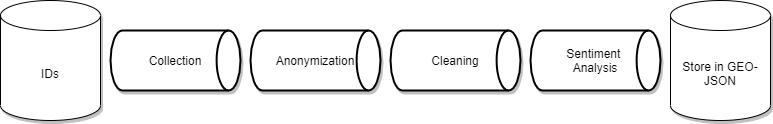
\includegraphics[width=\linewidth]{figures/data pipeline.png}
  \caption{A visualization of the pipeline, which we used for the pre-processing of our data}
  \label{fig:viz2}
\end{figure}
\label{data_prep}

Most microblogging services like \emph{Twitter} provide an API for data collection in combination with their policies.
To ensure integrity and safety of users data, firstly, the message authors have to be anonymized in such a way that no user could be identified via the dataset. Afterwards, additional preparation steps can be taken to prepare the data for analytical purposes. We will lay out the steps we took in our example, but explore additional possibilities later on. 

Our pipeline consists of following steps: Data collection, data anonymization, textual cleaning, sentiment analysis and data storage.
Data collection is done via the official Twitter API\footnote{\url{https://developer.twitter.com/en/docs/tools-and-libraries}} for Python, through which tweets can be selected by ID. We chose to focus on messages which talked about the COVID-19 pandemic, a dataset for which is provided by ~\cite{DVN/LW0BTB_2020}. After receiving the tweets through the API, the authors were replaced by randomized IDs, which were stored together with the message texts, IDs of targets, location and timestamp. Messages without any location or timestamp were removed, since they could not be visualized reasonably. 

To clean the textual data, we lower cased all letters and removed punctuation as well as special characters like emojis. This cleaned version is only used for the sentiment analysis later on. When showing the text to the user, we still use the original version. 

In our example, we chose to apply a sentiment analysis to the message texts, to show one additional dimension. Tools and resources for sentiment analysis are widely available, and we went with a simple transformer network provided by \url{https://github.com/chriskhanhtran/bert-for-sentiment-analysis}. Our sentiment analysis only consists of one dimension: Positivity of message. Examples for contents which make a message more negative would be usage of curse words, expression of negative emotions like anger. More positive messages contain expressions of happiness or gratitude. Each message gets evaluated individually and ranked on a scale from 0 to 1, with 0 being very negative and 1 being very positive. 

We store all these in formations inside a JSON-file. Since we are using the United States as our example location, we use individual states as keys, which map to Geo-JSON information, as well as a list of messages, each identified by ID and containing the collected information. For an explanation and further information on Geo-JSON, we refer to \cite{rfc7946}.

\section{Visualization} 
To start our visualization process, we first render a simple 2D map of the US with clear borders being visible. We then start to build objects, which hold the information necessary to ensure an effective visualization. For this we go through all entries in the Geo-JSON file, create a new object for every entry and copy the information from every entry into the corresponding object. We then continue to calculate the position of each object in the 3D-plot. While the X-and Y-coordinates can be derived from the state the message was posted in, the Y-coordinate stems from the order of dates, in the given state of the message. For example, if the message is the 5th message in the state, it will result in it's Y-coordinate being $5+x$ with $x:=$ $offset$ $between$ $points$. This is a rather rigid way of assigning coordinates, but making the Y-coordinate of every message depend directly on the absolute time it was posted at, could result in overlapping points and large gaps between points. The algorithm for this method can be found at \ref{alg:1}.

\begin{algorithm}[H]
 \KwData{Geo-JSON}
 \KwResult{List of visualizable objects}
 objects = newList() \; 
 \For{Country in JSON.keys()}{
   \For{Message in country}{
        messageObject = newObject() \;
        messageObject.information = Message.information \;
        messageObject.location = (Country.x, i + Message.index, Country.z)\;
        objects.add(messageObject) \;
 }
 }
 \label{alg:1}
 \caption{Conversion of Geo-JSON in visualizable objects}
\end{algorithm}

The final visualization step consists of actually rendering the \emph{messageObjects}. We went with an approach where every object was rendered as a simple, same-sized cube. Each cube would be colored according to the underlying sentiment value extracted from the post said cube represents. In our case, we selected green for more positive sentiments and red for more negative once, following mainstream coloring conventions. Since X-coordinates and Z-coordinates depend on the state the message was recorded in, and the Y-coordinate depends on how many messages were recorded before the current message, this results in columns of messages over each state, where all messages have an even amount of space to the respective cube above or under them. The final visualization should like \ref{fig:viz2}. 

\begin{figure}
  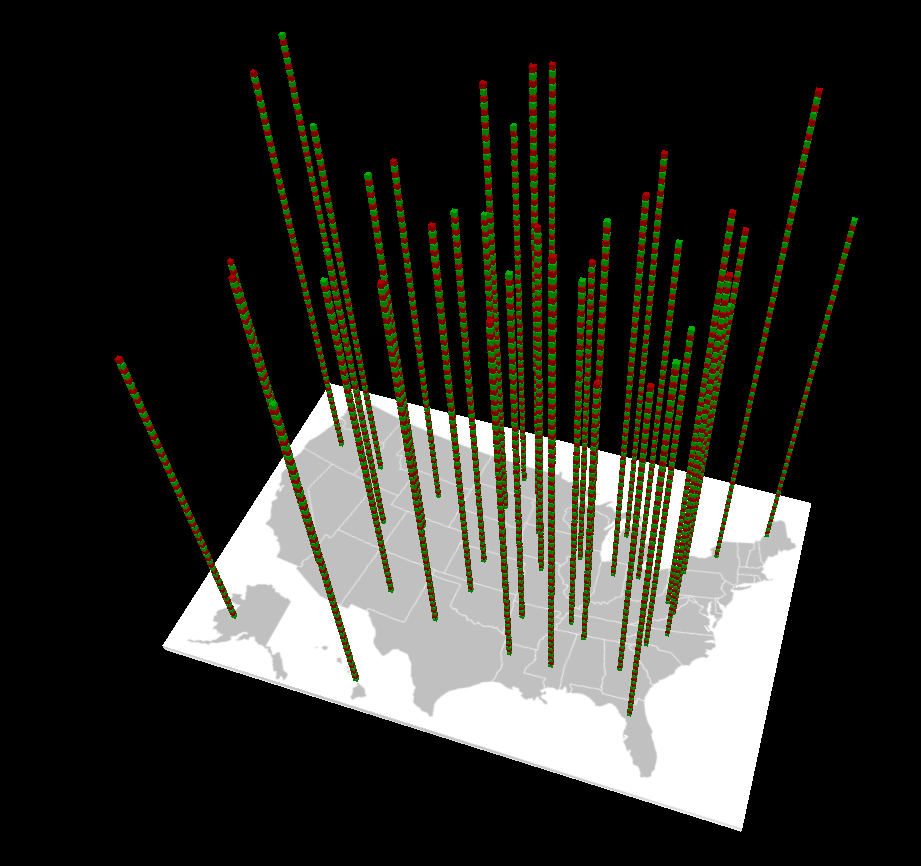
\includegraphics[width=\linewidth]{figures/viz3.PNG}
  \caption{Static visualization of message objects in time and space. Each column corresponds with the US state it stands on and goes forward in time from the bottom up. Therefore, each cube is a message in time and space.}
  \label{fig:viz2}
\end{figure}
After all the \emph{messageObjects} are visualized in this manner, we want to also show relationships between messages, to make it easier for the user, to follow conversational threads. After the user selects any \emph{messageObjects} he wants to understand more context of, we show the stream of conversation via arrows. If a post was done as a \emph{retweet} to another \emph{tweet}, an arrow is drawn from the cube, which represents the \emph{retweet}, to the one representing the original \emph{tweet}. This way the thread, which lead to the selected message, is opened up and can be analyzed by the user. An example for such a thread can be found at \ref{fig:viz4}.

\begin{figure}
  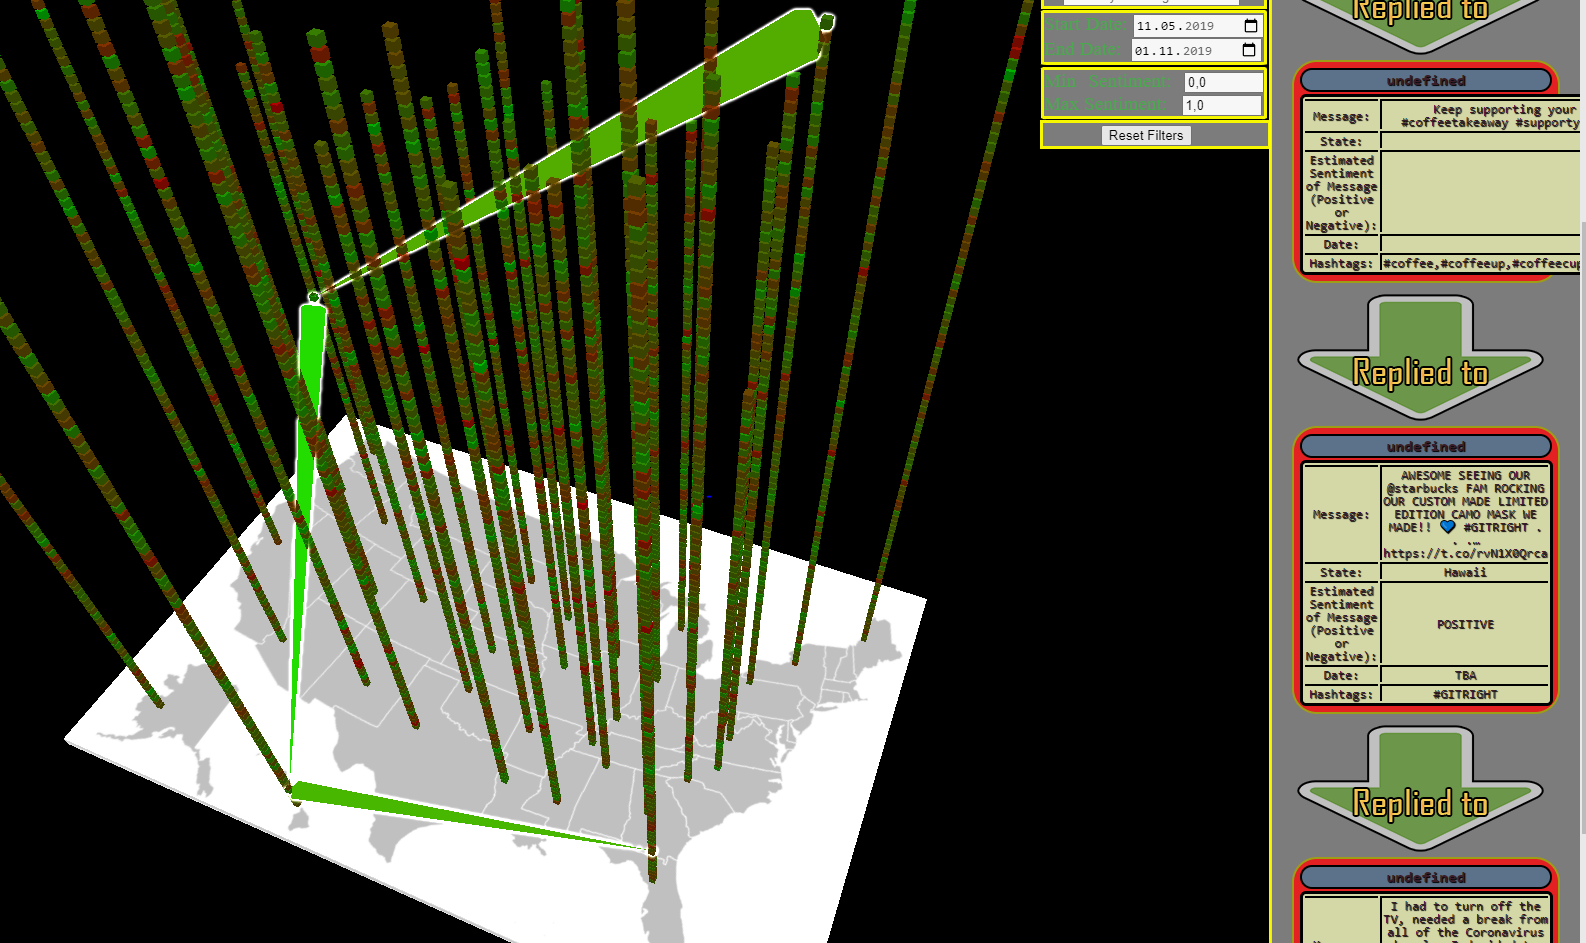
\includegraphics[width=\linewidth]{figures/example3.PNG}
  \caption{A typical conversational thread. The thread starts at the topmost cube and from there runs through arrows, which point from one message, to the message it is an answer to. The color of the arrow corresponds with the sentiment of the message, where green is positive and red is negative}
  \label{fig:viz4}
\end{figure}

\section{Filter}
To ensure that users may use the visualization, to answer specific research questions, we included the option to filter for individual criteria. Options for filtering include as follows:
\begin{itemize}
    \item Range of specific dates
    \item Range of sentiment values
    \item Inclusion of specific hashtags
    \item Exclusion of specific hashtags
\end{itemize}
This list is comprehensive of all possible options, and we strongly encourage the usage and inclusion of further possible filters, as more dimensions will be added to the visualization.
\section{Aggregate Visualization}
The basic 3D-rendering visualizes individual posts in a microblogging service and the relationship between them. It allows following conversational threads and not to get lost in a largely expanding conversational tree. However, broad overviews over different statistics can still be useful, when analyzing topics at hand. For this, we integrated a view with aggregated statistics over all available dimensions, which is visible in parallel to the rendering. An example for this view can be seen in \ref{fig:viz3}.
\begin{figure}
  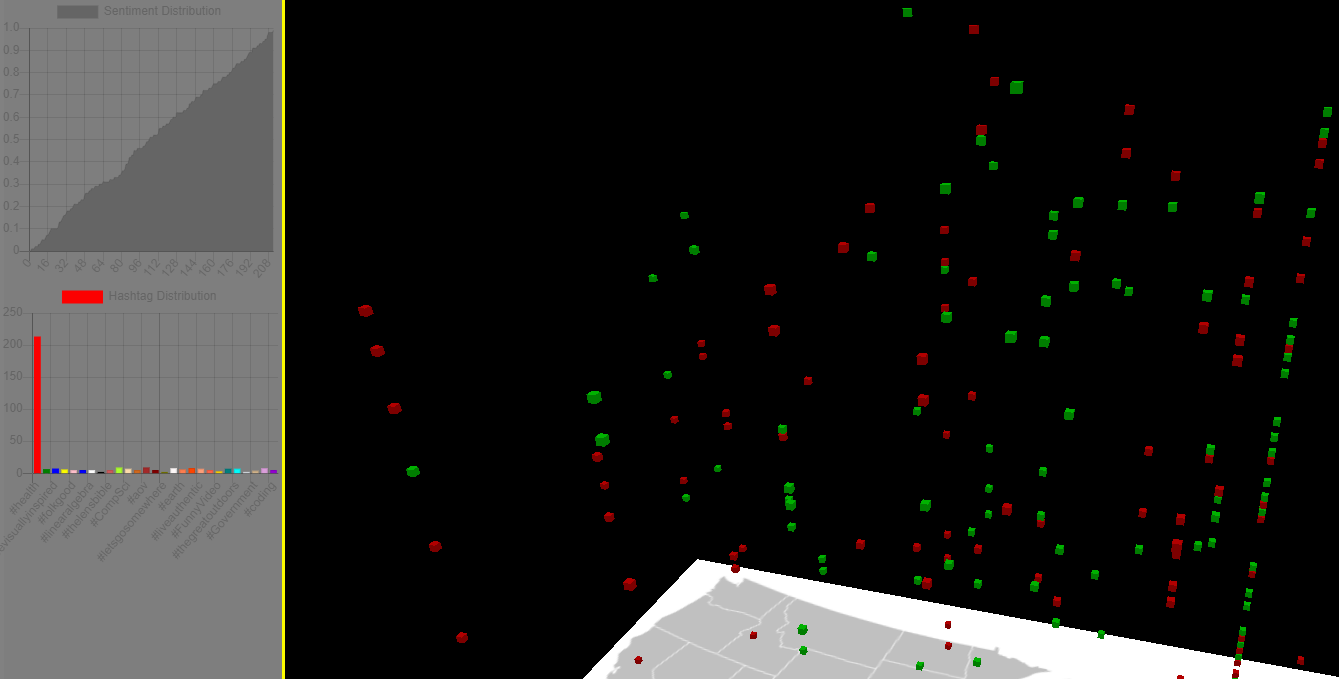
\includegraphics[width=\linewidth]{figures/stats.PNG}
  \caption{Rendering with statistics and filters applied. Only cubes are rendered, which do meet the requirements set by the filter. On the left, statistics over the sum of all rendered messages are shown.}
  \label{fig:viz3}
\end{figure}

This brings with it a few advantages. Firstly, it allows for more precise selection of filters, since one can directly see the effects which occur, when applying changes to any dimension. It also allows seeing a clearer picture of the discourse overall, contextualizing any single conversational thread, one is studying at the moment.
  \chapter{Implementation}
\label{imp}
% %%%%%%%%%%%%%%%%%%%%%%%%%%%%%%%%%%%%%%%%%%%%%%%%%%%%%%%%%%%%%%%%%%%%%%%%
\section{Tools}
To ensure cross-platform accessibility and ease-of-use, we chose to implement our demo in JavaScript for the usage in internet browsers. Not only can our demo be viewed under any operating system, but also through each device, which is able to use a browser software.

As a 3D-rendering tool, we went with the library three.js\footnote{\url{https://threejs.org/}}. For the display of statistics in graphs, we used chart.js\footnote{\url{https://www.chartjs.org/}}. Implementations through different technologies, programming languages and libraries, for different use-cases are also viable. If one wants to achieve faster real-time visualizations on bigger datasets, we recommend using C++ and rendering the visualization via \textit{OpenGL} and \textit{cpplot} for the creation of dynamic graphs.
\section{Technical Limits}
When implementing our visualization, we were faced with some technical issues, which we were not able to solve directly through optimization and which future research should aim to resolve. Firstly was the amount of RAM, which our method needs to function. This does mostly stem from the usage of Geo-JSON, but also from the other information, which we save, since we load the whole of the data into RAM directly. Often times this can lead to \emph{out-of-memory}-errors. Since we only want to show a demo of how our software could work, we resolved this by only using a limited amount of messages, to visualize at a time. A more sophisticated solution could entail the streaming of the data in a limited capacity at a time. This would reduce RAM usage, whilst still allowing to visualize a larger amount of data points. 

Further limitations arise from the Twitter-API itself. Even though it features a lot of great features and built-in support, it only allows the collection of a limited \emph{tweets} per hour. Since there is no real workaround for this issue, we recommend planning in a longer collection-period for messages.

The last major issue stems from the amount of messages, which can rendered meaningfully at a time. Because our tool should allow users to acquire an easily understandable overview of conversations, rendering every single message could be counterproductive, since it would lead to an overload of displayed information. As a further improvement, we propose the bulking of similar messages, which were posted in the same state, at roughly the same time period. Possible metrics for such a process could be based on the usage of same or similar \emph{hashtags}, or on methods from the area of Text Similarity.
  %%%%%%%%%%%%%%%%%%%%%%%%%%%%%%%%%%%%%%%%%%%%%%%%%%%%%%%%%%%%%%%%%%%%%%%%
\chapter{Results}
\label{chap:Results}

To show the viability of our tool in the field, we run a small-scale analysis on a small dataset, using a simple research question. We chose this limited approach due to our limited computational budget and time-constraints, but hope to try more in-depth looks in the future. 

For our research question we went with the following: "Are typical conversational threads, in the last three weeks, more negative over all, when looking at online discussions about computer science, in comparison to other topics?". We chose this question, since it follows our intended structure of trying to ask questions about conversational threads in subgroups of a larger conversational space online. Answering this question can be done through our tool as follows:
\begin{enumerate}
    \item Load appropriate data
    \item Filter for data from the last three weeks
    \item Follow typical conversational threads in the larger conversational space
    \item Filter for typical hashtags about computer science, like #computerscience or #CompSci
    \item Compare conversational threads to ones in the larger space
    \item Validate results through look on aggregated statistics
\end{enumerate} 


Finally, we can show unique and interesting findings, which would not have been possible to see without our tool. Figure \ref{fig:example1} shows a typical pattern, which we found often, when looking through the data. The debate, which is held in this thread about the COVID-19 pandemic, keeps a rather negative tone from the bottom up. The conversation however abruptly ends, when a positive connotated message is sent in the end, which can be seen through the bright, green arrow coming down from the top. This pattern of "positive-stops" can be seen in multiple instances and might be an interesting starting point for further research.

\begin{figure}
  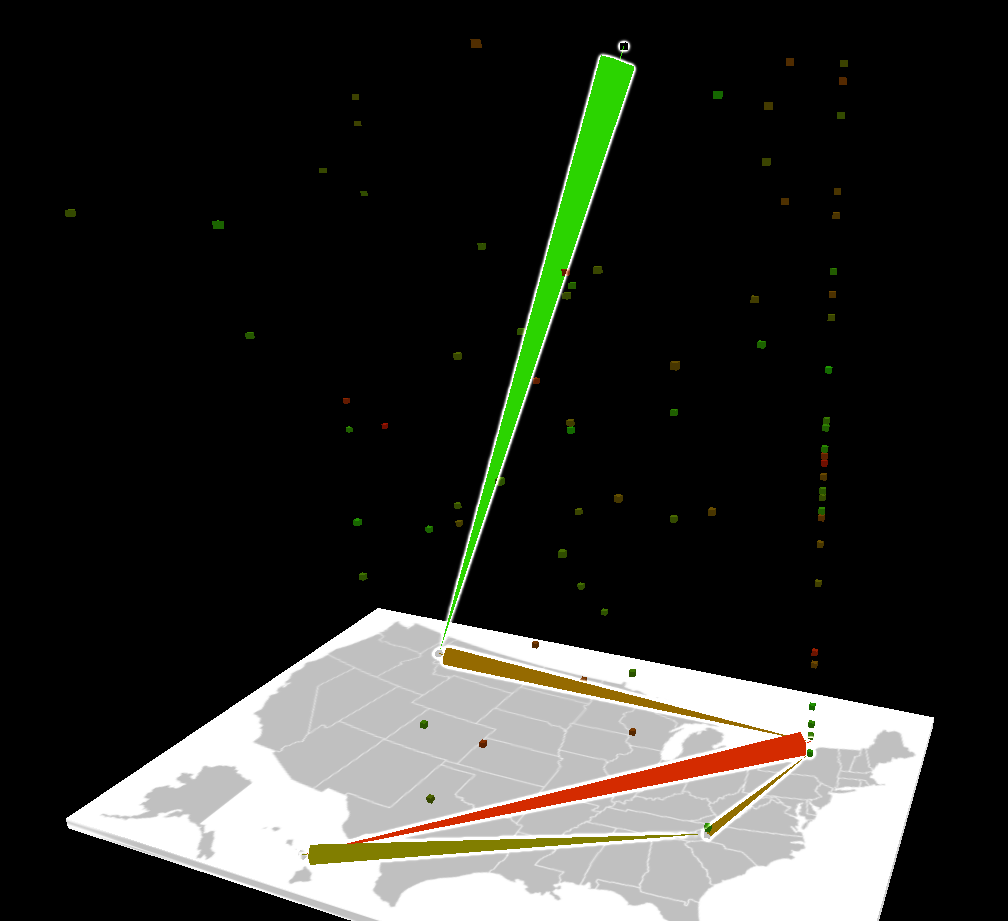
\includegraphics[width=\linewidth]{figures/exempleary.PNG}
  \caption{Rendering with statistics and filters applied. Only cubes are rendered, which do meet the requirements set by the filter. On the left, statistics over the sum of all rendered messages are shown.}
  \label{fig:example1}
\end{figure}
%%%%%%%%%%%%%%%%%%%%%%%%%%%%%%%%%%%%%%%%%%%%%%%%%%%%%%%%%%%%%%%%%%%%%%%%
  %%%%%%%%%%%%%%%%%%%%%%%%%%%%%%%%%%%%%%%%%%%%%%%%%%%%%%%%%%%%%%%%%%%%%%%%
\chapter{Conclusion}
We proposed a novel scheme for rendering diverse discussion threads on microblogging platforms, through which complex research questions, concerning the discussion, can be analyzed and answered. Our visualization can show temporal, spatial, sentimental and other dimensions at the same time, and reduce complexity for the user. Our combination of 3D-rendering of spatial and temporal data points with aggregated statistics and the option to introduce filters, allows for a very precise and in-depth answering of research questions, which can be proposed by users, who want to analyze specific aspects of conversations over microblogging sites. We also show a possible pipeline for preparing any data from a social media platform, for usage in our dashboard. Our experiments show, that this scheme can be used effectively to answer research questions about discourse online, while still minimizing the complexity in terms of visualization and user interface. Further research should try more complex questions on more complex data, to evaluate the possibilities further.  

Further research should look into ways of reducing the memory-complexity of our method, which is the main bottleneck right now, when trying to incorporate large amounts of data ($>3000$ data points) at once. Methods for streaming the data, instead of loading it into memory at once, could prove useful. Another task for further exploration could be the incorporation of additional visualization methods for different dimensions. Methods from fields like optical flow could be used to indicate changes in values over time and/or space very intuitively. Finally, improvements in the modularity of our tool would be highly welcome. Right now, it is focused on visualizing spatial data from the United States. A procedural approach for rendering maps on different scales on the fly, would make it so that discourse over international borders could be analyzed more easily. Additionally, looking into ways of tracking the flow of different topics in conversations could be worthwhile. One could for example filter for change of topics in conversational threads and correlating changes in e.g. sentiments or other variables.
To further possible insights into how to improve our methods, we strongly encourage the usage of our tools in fields like political science or communications, for analysis of online discourse.
%%%%%%%%%%%%%%%%%%%%%%%%%%%%%%%%%%%%%%%%%%%%%%%%%%%%%%%%%%%%%%%%%%%%%%%%  

% This ensures that the subsequent sections are being included as root
% items in the bookmark structure of your PDF reader.
\bookmarksetup{startatroot} 
\backmatter

  \printindex
  \label{sec:index}
  
  \printbibliography
  
\end{document}